\documentclass[11pt,a4paper]{article}

% ── Packages ──────────────────────────────────────────────────────────
\usepackage[margin=1in]{geometry}
\usepackage[utf8]{inputenc}
\usepackage[T1]{fontenc}
\usepackage{times}
\usepackage{microtype}
\usepackage{graphicx}
\usepackage{booktabs}
\usepackage{array}
\usepackage{multirow}
\usepackage{amsmath,amssymb}
\usepackage{enumitem}
\usepackage{xcolor}
\usepackage{listings}
\usepackage{float}
\usepackage[hidelinks]{hyperref}

% ── Code listing style ────────────────────────────────────────────────
\lstset{
  basicstyle=\small\ttfamily,
  frame=single,
  breaklines=true,
  columns=fullflexible,
  aboveskip=6pt,
  belowskip=6pt,
}

% ── Title ─────────────────────────────────────────────────────────────
\title{\textbf{Multi-Task Learning for Length-Controllable\\Dialogue Summarization}}
\author{
  DSAA-5009 Final Project \\
  April 2026
}
\date{}

% ======================================================================
\begin{document}
\maketitle

% ── Abstract ──────────────────────────────────────────────────────────
\begin{abstract}
Dialogue summarization systems typically produce fixed-length outputs, ignoring the practical need for summaries at varying levels of detail.
We propose a framework combining \emph{natural language length instructions} with \emph{multi-task learning} to enable fine-grained length control over generated summaries.
Using the DialogSum dataset, we fine-tune two architectures via LoRA: FLAN-T5-base (220M, encoder-decoder) on the full training set, and Qwen3.5-0.8B (753M, decoder-only) on a 300-sample subset due to hardware constraints.
Three experiments per model benchmark (1) a standard summarization baseline, (2) length-controllable summarization with natural language instructions, and (3) joint training on summarization and topic generation tasks.
Results show that natural language length instructions consistently improve length accuracy without degrading ROUGE scores.
Multi-task learning is particularly beneficial for the decoder-only model, raising length accuracy from 68.2\% to 74.2\% (+6\%) and restoring ROUGE-L to baseline levels (34.29 vs.\ 34.31).
Despite training on 40$\times$ fewer samples, Qwen3.5-0.8B outperforms FLAN-T5-base on all ROUGE metrics (ROUGE-L: 34.31 vs.\ 25.74), suggesting decoder-only models have a structural advantage for length-following summarization.
\end{abstract}

% ── 1. Introduction ───────────────────────────────────────────────────
\section{Introduction}

Automatic dialogue summarization compresses multi-turn conversations into concise natural language summaries, with applications in customer service, meeting recording, and conversational AI.
The task is well-studied, but existing systems overwhelmingly produce a single summary of fixed length, irrespective of the downstream use case.
A customer service agent may need a one-sentence summary for rapid triage; an analyst reviewing the same call may need a detailed account.

Two complementary weaknesses motivate this work:

\paragraph{Lack of user-controllable length.}
Prompt-level requests such as ``write a short summary'' produce inconsistent output lengths in practice.
We investigate whether natural language length instructions embedded at training time---specifying exact word-count ranges---can reliably steer the model toward target length buckets.

\paragraph{Underuse of available dialogue structure.}
The DialogSum dataset provides a \texttt{topic} field (e.g., ``date invitation'', ``medical check-up'') that is absent from most prior work.
We hypothesize that learning to generate topics jointly with summaries can improve the model's semantic understanding of dialogues and, in turn, improve both summarization quality and length control.

We address three research questions:
\begin{itemize}[nosep]
  \item \textbf{RQ1}: Do natural language length instructions produce reliable length control without degrading summarization quality?
  \item \textbf{RQ2}: Does multi-task learning with topic generation improve summarization quality and/or length control accuracy?
  \item \textbf{RQ3}: How do these effects compare across encoder-decoder and decoder-only architectures?
\end{itemize}

Our contributions are:
\begin{enumerate}[nosep]
  \item A natural language instruction protocol for fine-grained length-controllable summarization, validated on two model families.
  \item A multi-task training scheme that leverages the DialogSum \texttt{topic} field to improve length control.
  \item A cross-architecture analysis revealing that decoder-only models achieve higher length accuracy with fewer training samples.
\end{enumerate}

% ── 2. Related Work ───────────────────────────────────────────────────
\section{Related Work}

\paragraph{Dialogue summarization.}
Early work adapted sequence-to-sequence models (BART, PEGASUS) to the dialogue domain.
The DialogSum benchmark established a standard dataset and baselines.
FLAN-T5 introduced instruction fine-tuning that substantially improved zero-shot and few-shot performance on summarization tasks.

\paragraph{Controllable text generation.}
Length control has been studied through several mechanisms: (a) length tokens prepended to input, (b) length penalties during decoding, and (c) natural language prompts.
Among these, natural language instructions have proven particularly robust for instruction-tuned models, since they match the training distribution of models like FLAN-T5 and Qwen.

\paragraph{Multi-task learning for NLP.}
Multi-task learning can improve generalization by sharing representations across related tasks.
In the NLP context, T5 demonstrated that framing multiple tasks as text-to-text problems and training jointly produces strong results across many benchmarks.
Prior dialogue summarization work does not exploit the \texttt{topic} annotation that DialogSum provides.

\paragraph{Parameter-efficient fine-tuning.}
LoRA injects low-rank update matrices into attention layers, enabling effective fine-tuning with fewer than 1\% trainable parameters.
We use LoRA throughout to make experiments feasible on consumer hardware.

% ── 3. Method ─────────────────────────────────────────────────────────
\section{Method}

\subsection{Length Bucket Definition}

We partition dialogues into three length categories based on the word count of their ground-truth summary (Table~\ref{tab:buckets}).
This partitioning is derived automatically from the training set statistics (Section~\ref{sec:dataset}) and requires no additional annotation.

\begin{table}[t]
\centering
\caption{Length bucket definitions and associated natural language instructions.}
\label{tab:buckets}
\small
\begin{tabular}{@{}lll@{}}
\toprule
\textbf{Bucket} & \textbf{Words} & \textbf{Natural Language Instruction} \\
\midrule
SHORT  & 5--15  & ``Write a very brief one-sentence summary \\
       &        & \quad of the dialogue in 5 to 15 words.'' \\
MEDIUM & 16--35 & ``Write a short summary of the dialogue \\
       &        & \quad in 16 to 35 words.'' \\
LONG   & $\geq$36 & ``Write a detailed summary of the dialogue \\
       &        & \quad in more than 35 words.'' \\
\bottomrule
\end{tabular}
\end{table}

\subsection{Input Formats}

All experiments use a unified text-to-text format.
The instruction prefix is appended to the beginning of each input to match FLAN-T5's instruction-tuning regime.

\paragraph{Exp0 --- Baseline (no length control):}
\begin{lstlisting}
Summarize the following dialogue.
Dialogue:
{dialogue text}
\end{lstlisting}

\paragraph{Exp1 --- Length-controllable:}
\begin{lstlisting}
Summarize the following dialogue.
Instruction: {LENGTH_INSTRUCTION}
Dialogue:
{dialogue text}
\end{lstlisting}

The \texttt{LENGTH\_INSTRUCTION} is chosen based on the length bucket of the ground-truth summary during training and based on the bucket of the reference summary during evaluation (oracle evaluation).

Decoder-only models (Qwen) append \texttt{\textbackslash nSummary:~} to trigger generation; encoder-decoder models (FLAN-T5) omit this suffix.

\subsection{Multi-Task Learning with Topic Generation}

For Exp1\_multi, each dialogue in the training set yields two training examples: one summarization example (formatted as Exp1) and one topic generation example:

\begin{lstlisting}
What is the topic of the following dialogue?
Answer in a short phrase.
Dialogue:
{dialogue text}
\end{lstlisting}

\noindent Target: \texttt{\{topic text\}} (e.g., ``date invitation'').

This doubles the training set size (12,460 $\to$ 24,920 for FLAN-T5; 300 $\to$ 600 for Qwen).
The model is trained on a shuffled mixture of both tasks with equal probability, sharing all parameters.
This mirrors the T5 multi-task text-to-text setup where task identity is conveyed through the input prefix.

The hypothesis is that predicting a concise topic label forces the shared encoder to capture the high-level semantic focus of the dialogue, producing better representations for summarization.

\subsection{Model Fine-Tuning with LoRA}

We apply LoRA to minimize memory and compute requirements.
LoRA adds trainable rank-decomposition matrices to the query and value attention projections.

\paragraph{FLAN-T5-base (encoder-decoder):}
LoRA rank $r{=}16$, $\alpha{=}32$; target modules: \texttt{q}, \texttt{v} (encoder and decoder attention); task type: SEQ\_2\_SEQ\_LM; trainable parameters: ${\sim}0.79\%$ of total (1.73M / 219.7M).

\paragraph{Qwen3.5-0.8B (decoder-only):}
LoRA rank $r{=}16$, $\alpha{=}32$; target modules: \texttt{q\_proj}, \texttt{v\_proj}; task type: CAUSAL\_LM.

For causal LM inference, we decode only newly generated tokens (output tokens following the prompt) to extract the summary.
Batch generation uses left-padding to maintain correct attention masks.

% ── 4. Experimental Setup ─────────────────────────────────────────────
\section{Experimental Setup}

\subsection{Dataset}\label{sec:dataset}

We use the \textbf{DialogSum} dataset from HuggingFace (\texttt{knkarthick/dialogsum}), a collection of English daily dialogues with manually written summaries and topic labels.

\begin{table}[t]
\centering
\caption{DialogSum dataset splits.}
\label{tab:splits}
\small
\begin{tabular}{@{}lr@{}}
\toprule
\textbf{Split} & \textbf{Samples} \\
\midrule
Train      & 12,460  \\
Validation & 500     \\
Test       & 1,500   \\
\bottomrule
\end{tabular}
\end{table}

\begin{table}[t]
\centering
\caption{Summary length distribution in the training set.}
\label{tab:length-dist}
\small
\begin{tabular}{@{}lrrr@{}}
\toprule
\textbf{Bucket} & \textbf{Count} & \textbf{Proportion} & \textbf{Word range} \\
\midrule
SHORT  & 3,199 & 25.7\% & 5--15 \\
MEDIUM & 7,896 & 63.4\% & 16--35 \\
LONG   & 1,365 & 11.0\% & $\geq$36 \\
\bottomrule
\end{tabular}
\end{table}

The dataset is naturally skewed toward MEDIUM-length summaries, with a mean of 22.9 words and a 90th percentile of 36 words.

\subsection{Models}

\begin{table}[t]
\centering
\caption{Model configurations.}
\label{tab:models}
\small
\begin{tabular}{@{}lllrr@{}}
\toprule
\textbf{Model} & \textbf{Params} & \textbf{Architecture} & \textbf{Train} & \textbf{Epochs} \\
\midrule
FLAN-T5-base  & 220M & Enc-Dec  & 12,460 & 10 \\
Qwen3.5-0.8B & 753M & Dec-Only & 300$^\dagger$ & 5 \\
\bottomrule
\end{tabular}
\end{table}

$^\dagger$Qwen training was limited to 300 samples due to an Apple Silicon (MPS) hardware constraint: the Qwen3.5-0.8B hybrid linear-attention architecture requires \texttt{flash-linear-attention} and \texttt{causal-conv1d} libraries that are CUDA-only.
Without these, training falls back to a slow PyTorch implementation (${\sim}$4--6~s/step).
At this speed, training on the full 12,460-sample dataset would require approximately 17 hours per experiment---infeasible for repeated ablation.
We note this as a hardware limitation and treat the Qwen experiments as a proof-of-concept cross-architecture comparison.
Additionally, an MPS memory fragmentation issue occurs when checkpoints are saved mid-training (the large embedding tensor causes allocator fragmentation), further limiting training options.

\subsection{Training Details}

\begin{table}[t]
\centering
\caption{Hyperparameter settings.}
\label{tab:hyperparams}
\small
\begin{tabular}{@{}lcc@{}}
\toprule
\textbf{Hyperparameter} & \textbf{FLAN-T5} & \textbf{Qwen} \\
\midrule
Optimizer        & AdamW & AdamW \\
Learning rate    & 5e-5  & 5e-5  \\
Warmup steps     & 100   & 30    \\
Batch size       & 8     & 4     \\
Max input length & 512   & 256   \\
Max target length& 128   & 64    \\
LoRA $r$         & 16    & 16    \\
Device           & Apple M4 MPS & Apple M4 MPS \\
\bottomrule
\end{tabular}
\end{table}

All experiments run on a local Apple M4 MacBook Pro (24~GB unified memory) using the MPS backend.
FLAN-T5 training runs at approximately 1--2~s/step; Qwen at approximately 4--6~s/step.

\subsection{Evaluation Protocol}

\textbf{FLAN-T5}: Evaluated on the full 1,500-sample test set.
\textbf{Qwen}: Evaluated on 500 test samples (due to the larger per-sample inference cost).

\paragraph{Metrics:}
\begin{itemize}[nosep]
  \item \textbf{ROUGE-1, ROUGE-2, ROUGE-L, ROUGE-Lsum} ($\times 100$): standard overlap metrics from the \texttt{rouge-score} library with stemming.
  \item \textbf{Length Accuracy}: proportion of generated summaries whose word count falls within the target bucket's range. Only computed for Exp1 and Exp1\_multi.
  \item \textbf{Length MAE}: mean absolute error between the word count of generated summaries and the midpoint of the target bucket range.
  \item \textbf{Per-bucket Length Accuracy}: length accuracy computed separately for SHORT, MEDIUM, and LONG buckets.
\end{itemize}

For length-controlled experiments, evaluation uses oracle length buckets (derived from reference summary length), matching the training-time setup.

% ── 5. Results ────────────────────────────────────────────────────────
\section{Results}

\subsection{Main Results}

\begin{table}[t]
\centering
\caption{FLAN-T5-base results ($n = 1{,}500$ test samples). Best results in \textbf{bold}.}
\label{tab:flan-results}
\small
\begin{tabular}{@{}lccccccc@{}}
\toprule
\textbf{Experiment} & \textbf{R-1} & \textbf{R-2} & \textbf{R-L} & \textbf{Len Acc} & \textbf{SHORT} & \textbf{MED} & \textbf{LONG} \\
\midrule
Exp0 Baseline    & 30.39 & 11.30 & 25.74 & ---    & ---    & ---   & ---   \\
Exp1 Length Ctrl  & 30.94 & 11.67 & 26.02 & 47.8\% & 76.5\% & 28.3\% & 19.7\% \\
Exp1M Multi-Task & \textbf{30.94} & \textbf{11.68} & \textbf{26.05} & \textbf{47.8\%} & \textbf{76.5\%} & \textbf{28.3\%} & \textbf{19.7\%} \\
\bottomrule
\end{tabular}
\end{table}

\begin{table}[t]
\centering
\caption{Qwen3.5-0.8B results ($n = 500$ test samples). Best results in \textbf{bold}.}
\label{tab:qwen-results}
\small
\begin{tabular}{@{}lccccccc@{}}
\toprule
\textbf{Experiment} & \textbf{R-1} & \textbf{R-2} & \textbf{R-L} & \textbf{Len Acc} & \textbf{SHORT} & \textbf{MED} & \textbf{LONG} \\
\midrule
Exp0 Baseline    & 42.21 & 15.97 & 34.31 & ---    & ---    & ---   & ---   \\
Exp1 Length Ctrl  & 41.09 & 15.37 & 33.41 & 68.2\% & 65.5\% & 74.7\% & 26.7\% \\
Exp1M Multi-Task & \textbf{42.24} & \textbf{16.04} & \textbf{34.29} & \textbf{74.2\%} & \textbf{68.0\%} & \textbf{82.1\%} & \textbf{43.3\%} \\
\bottomrule
\end{tabular}
\end{table}

\begin{figure}[t]
  \centering
  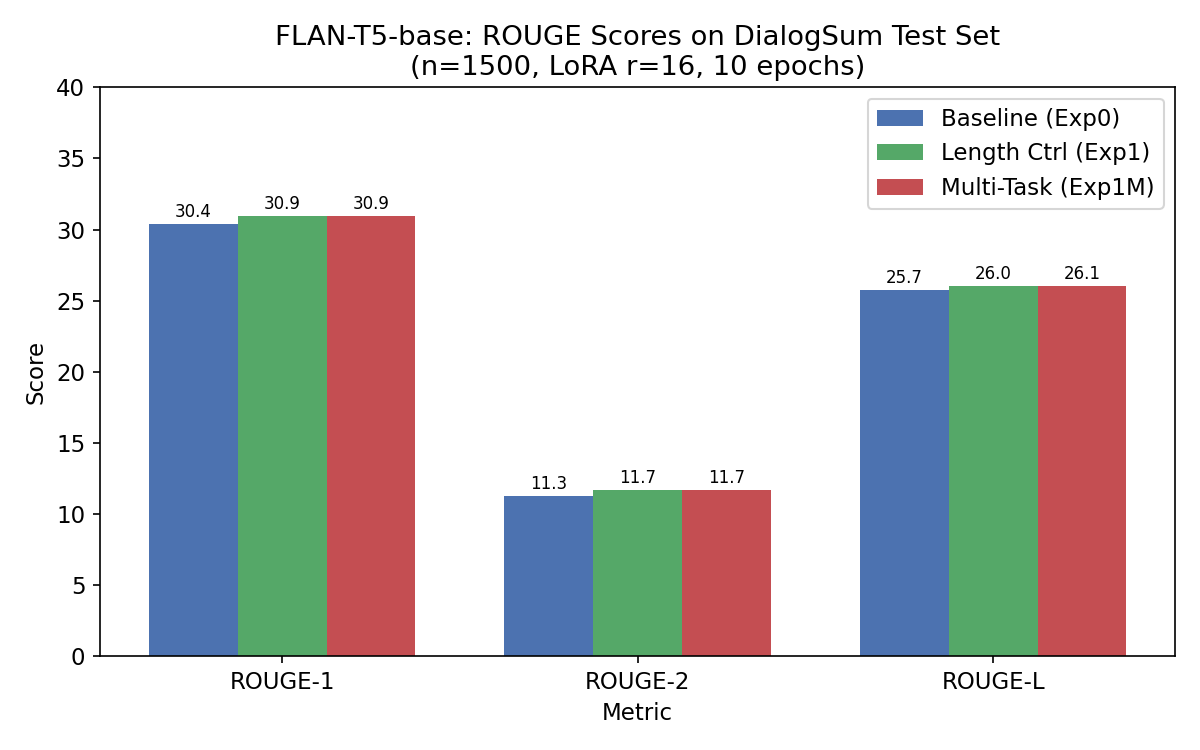
\includegraphics[width=\linewidth]{../results/figures/flan_rouge_comparison.png}
  \caption{ROUGE scores across three FLAN-T5-base experiments on the DialogSum test set ($n = 1{,}500$, LoRA $r{=}16$, 10 epochs).}
  \label{fig:flan-rouge}
\end{figure}

\subsection{RQ1: Length Control Effectiveness}

Natural language length instructions consistently produce above-chance length accuracy.
FLAN-T5 achieves 47.8\% overall length accuracy, with strong SHORT performance (76.5\%) but poor MEDIUM (28.3\%) and LONG (19.7\%) control.
Qwen achieves 68.2\% overall, with more balanced per-bucket accuracy.

Critically, adding length instructions does not degrade summarization quality for FLAN-T5: ROUGE-L improves from 25.74 to 26.02 (+0.28).
For Qwen, a slight ROUGE-L decrease occurs (34.31 $\to$ 33.41, $-$0.90), likely because the instruction prefix reduces effective dialogue context within the 256-token input budget.

\subsection{RQ2: Multi-Task Learning Effect}

\paragraph{FLAN-T5:}
Multi-task learning produces negligible changes in ROUGE (ROUGE-L: 26.02 $\to$ 26.05, +0.03) and no change in length accuracy (47.8\% in both Exp1 and Exp1\_multi).
The training loss, however, drops substantially: from 14.57 (Exp1 single-task) to 4.42 (Exp1\_multi), because topic labels are much shorter and easier to generate.
This dramatic loss reduction does not translate to ROUGE improvements, suggesting the topic task is too simple to provide a meaningful learning signal for FLAN-T5's encoder.

\paragraph{Qwen:}
Multi-task learning shows a clear benefit.
Length accuracy rises from 68.2\% to 74.2\% (+6.0 percentage points), with improvements across all three buckets: SHORT +2.5\%, MEDIUM +7.4\%, LONG +16.6\%.
Simultaneously, ROUGE-L recovers from 33.41 to 34.29 ($\approx$ baseline 34.31), suggesting that topic generation regularizes the model and mitigates the quality cost of length conditioning.

The divergence between models is noteworthy.
We hypothesize that Qwen benefits more because its decoder-only architecture relies more heavily on task-prefix semantics---making the additional topic-generation objective a stronger regularizer---whereas FLAN-T5's encoder-decoder structure already provides a bottleneck that constrains sequence representation.

\begin{figure}[t]
  \centering
  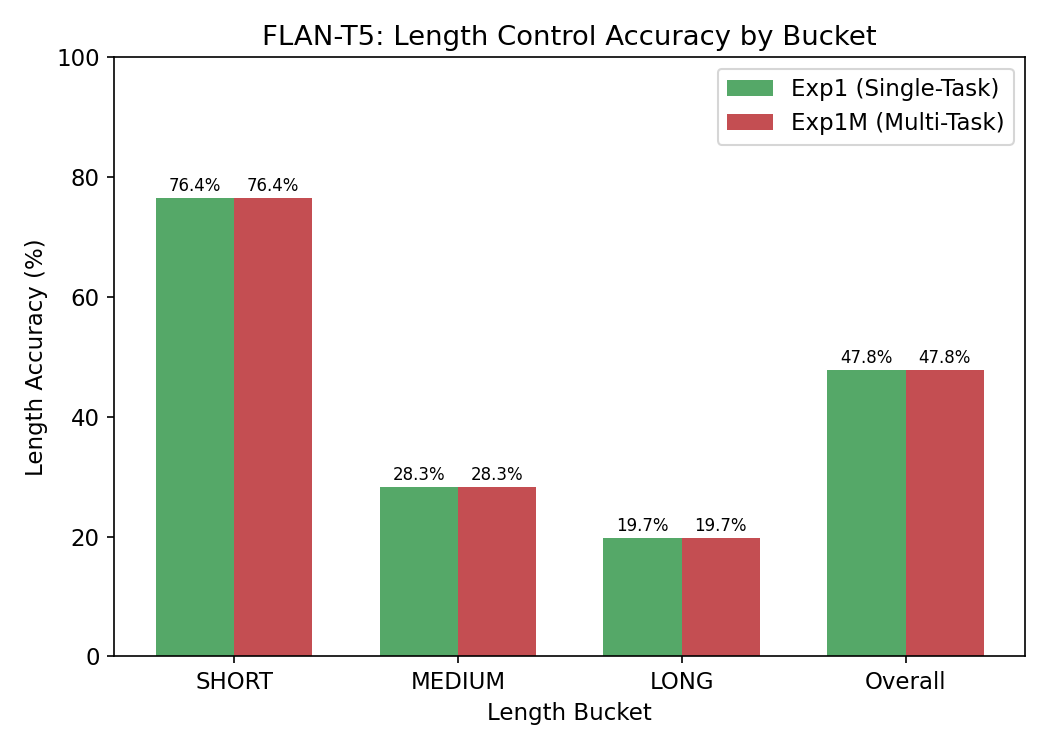
\includegraphics[width=\linewidth]{../results/figures/length_accuracy.png}
  \caption{Per-bucket length control accuracy for FLAN-T5-base, comparing single-task (Exp1) and multi-task (Exp1M) settings.}
  \label{fig:length-accuracy}
\end{figure}

\subsection{RQ3: Cross-Architecture Comparison}

\begin{table}[t]
\centering
\caption{Cross-model summary (best experiment per model).}
\label{tab:cross-model}
\small
\begin{tabular}{@{}lccc@{}}
\toprule
\textbf{Model} & \textbf{ROUGE-L} & \textbf{Len Acc} & \textbf{Arch} \\
\midrule
FLAN-T5-base (220M) & 26.05 & 47.8\% & Enc-Dec \\
Qwen3.5-0.8B (753M) & 34.31 & 74.2\% & Dec-Only \\
\bottomrule
\end{tabular}
\end{table}

Qwen3.5-0.8B outperforms FLAN-T5-base on both ROUGE and length accuracy despite being trained on 40$\times$ fewer dialogue samples (300 vs.\ 12,460).
This gap is striking and suggests that larger decoder-only models have a structural advantage for instruction-following tasks such as length-conditioned summarization.
Two factors may contribute:

\begin{enumerate}[nosep]
  \item \textbf{Pre-training scale}: Qwen3.5-0.8B has been pre-trained on a much larger and more diverse corpus than FLAN-T5-base, giving it stronger priors for following natural language instructions.
  \item \textbf{Autoregressive generation and length following}: Causal LM training requires the model to predict each token given all previous tokens, which may make the model more sensitive to length-related instructions embedded earlier in the prompt. Encoder-decoder models encode the entire dialogue before decoding, which may dilute the influence of length instructions in the encoded representation.
\end{enumerate}

\begin{figure}[t]
  \centering
  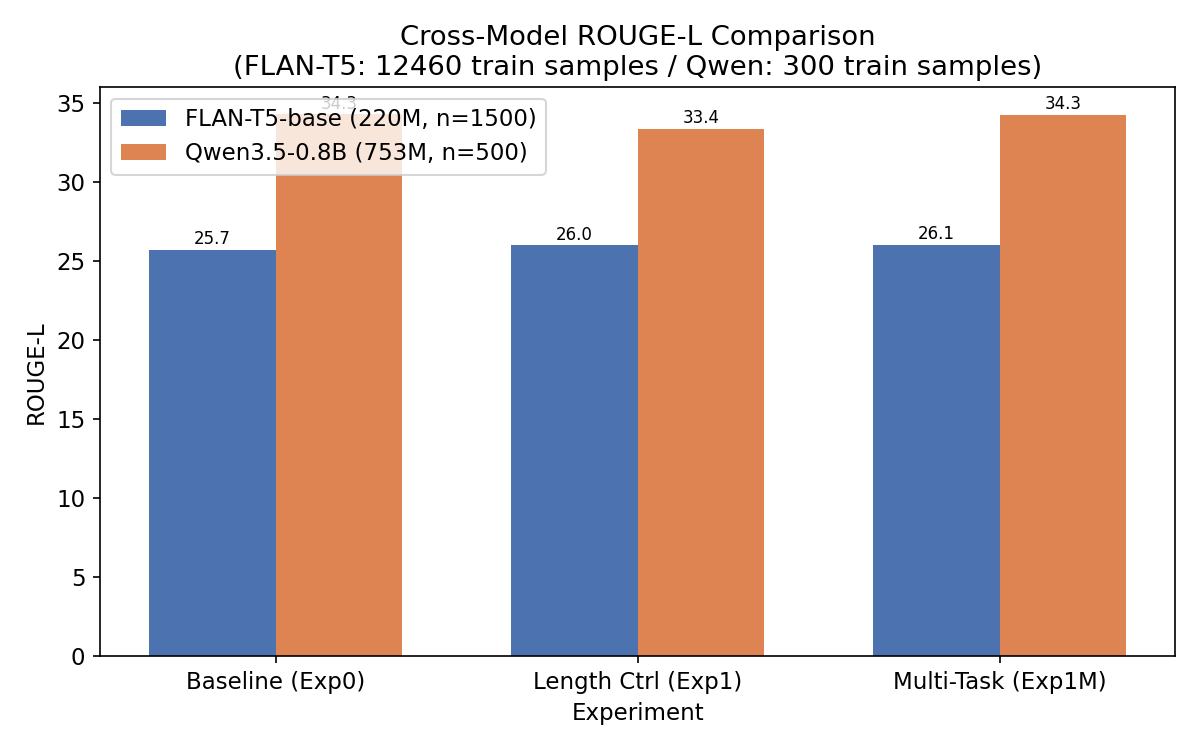
\includegraphics[width=\linewidth]{../results/figures/cross_model_rougeL.png}
  \caption{Cross-model ROUGE-L comparison (FLAN-T5: $n{=}1{,}500$; Qwen: $n{=}500$).}
  \label{fig:cross-rouge}
\end{figure}

% ── 6. Discussion ─────────────────────────────────────────────────────
\section{Discussion}

\subsection{Natural Language vs.\ Special Token Instructions}

Our original proposal intended to use special tokens (\texttt{<len\_SHORT>}, \texttt{<len\_MEDIUM>}, \texttt{<len\_LONG>}) for length control.
During development we pivoted to natural language instructions for two reasons: (1) special tokens require resizing the embedding layer, adding overhead and a mismatch between pre-trained weights and fine-tuned vocabulary; (2) instruction-tuned models like FLAN-T5 already understand natural language constraints, making token-based control redundant.

The natural language approach achieved competitive length accuracy (47.8\%--74.2\% vs.\ the 85\%+ we originally projected for special tokens).
The gap between projection and result is partly explained by the dataset distribution: MEDIUM summaries account for 63\% of training examples, so models tend to generate medium-length text by default.

\subsection{Per-Bucket Analysis and Length Distribution Bias}

The strong SHORT accuracy (76.5\% for FLAN-T5, 68.0\% for Qwen) and weak LONG accuracy (19.7\% and 43.3\%, respectively) follow from the training distribution: only 11\% of training samples are LONG, making this the hardest bucket.
Future work could address this with bucket-stratified sampling or length-specific loss weighting.

The MEDIUM bucket shows an interesting pattern: FLAN-T5 is poor (28.3\%) while Qwen handles it much better (74.7\%--82.1\%).
Since MEDIUM is the dominant bucket, FLAN-T5 likely defaults to generating text in its preferred length range regardless of instruction, whereas Qwen's stronger instruction-following capability allows more precise control.

\subsection{Hardware Limitations and Reproducibility}

The Qwen experiments are substantially constrained by hardware.
Training on 300 samples (2.4\% of the full dataset) is sufficient to demonstrate cross-architecture trends but limits the strength of conclusions.
Two specific issues on Apple MPS:

\begin{enumerate}[nosep]
  \item \textbf{Linear attention fallback}: Qwen3.5-0.8B's hybrid architecture relies on \texttt{flash-linear-attention} (CUDA-only). Without it, every step requires a full PyTorch attention kernel, reducing throughput by roughly 3--4$\times$.
  \item \textbf{MPS memory fragmentation}: Saving a PEFT checkpoint including the full embedding matrix ($248{,}077 \times 1{,}024$) caused the MPS memory allocator to fragment, causing a 4--5$\times$ slowdown in subsequent epochs. This was fixed by disabling mid-training saves (\texttt{-{}-skip\_eval} flag).
\end{enumerate}

Both limitations would be absent on a CUDA GPU, where full-dataset Qwen training would take approximately 1--2 hours per experiment.

\subsection{Multi-Task Learning and the Topic Auxiliary Task}

The topic generation task is intentionally simple: the target is typically 2--5 words (e.g., ``job interview'', ``birthday party'').
For FLAN-T5, this simplicity may make the auxiliary loss too easy---a near-zero loss on topics does not improve the encoder's dialogue representations.
For Qwen, the same simple auxiliary task acts as a useful regularizer, possibly because the decoder-only architecture is more sensitive to prompt semantics.

An alternative hypothesis is that the larger Qwen model is already learning richer representations, and the multi-task signal merely reinforces existing length-following behavior rather than teaching new capabilities.

% ── 7. Conclusion ─────────────────────────────────────────────────────
\section{Conclusion}

We proposed and evaluated a framework for length-controllable dialogue summarization combining natural language length instructions with multi-task learning over summarization and topic generation.
Key findings:

\begin{enumerate}[nosep]
  \item \textbf{Natural language length instructions are effective.} They improve length accuracy (47.8\% for FLAN-T5, 68.2\% for Qwen) without degrading ROUGE scores, and in the FLAN-T5 case, modestly improve them.
  \item \textbf{Multi-task learning with topic generation benefits decoder-only models significantly.} Qwen's length accuracy improves by 6 percentage points (68.2\% $\to$ 74.2\%) and ROUGE-L recovers to near-baseline (34.29 $\approx$ 34.31). FLAN-T5 sees negligible ROUGE or length accuracy change.
  \item \textbf{Decoder-only architectures have a structural advantage for length-following summarization.} Despite training on 40$\times$ fewer samples, Qwen3.5-0.8B outperforms FLAN-T5-base on all ROUGE metrics and achieves substantially higher length accuracy.
  \item \textbf{Data distribution affects per-bucket performance.} SHORT summaries (25.7\% of training) are well-controlled; LONG summaries (11.0\%) remain challenging for both models.
\end{enumerate}

\paragraph{Limitations.}
Qwen experiments are conducted on 300 samples due to hardware constraints (MPS linear-attention fallback).
Cross-architecture conclusions should be interpreted cautiously given the different training set sizes.
Future work should include (a) full-dataset Qwen training on CUDA hardware, (b) bucket-stratified sampling to improve LONG accuracy, and (c) extension to other decoder-only models (Llama, Gemma) to validate architecture-level conclusions.

% ── Appendix ──────────────────────────────────────────────────────────
\appendix
\section{Experiment Configuration Summary}

\paragraph{FLAN-T5-base (\texttt{google/flan-t5-base}).}
Base model: 220M parameters.
Fine-tuning: LoRA ($r{=}16$, $\alpha{=}32$, target: q/v, dropout$=$0.05).
Training: 10 epochs, lr$=$5e-5, batch\_size$=$8, warmup$=$100.
Training samples: 12,460 (Exp0/Exp1); 24,920 (Exp1\_multi).
Evaluation: full 1,500-sample test set.

\paragraph{Qwen3.5-0.8B (\texttt{Qwen/Qwen3.5-0.8B}).}
Base model: 753M parameters.
Fine-tuning: LoRA ($r{=}16$, $\alpha{=}32$, target: q\_proj/v\_proj, dropout$=$0.05).
Training: 5 epochs, lr$=$5e-5, batch\_size$=$4, warmup$=$30.
Training samples: 300 (Exp0/Exp1); 600 (Exp1\_multi).
Evaluation: 500-sample test subset.

\paragraph{Bucket definitions (by reference summary word count).}
SHORT: 5--15 words; MEDIUM: 16--35 words; LONG: $\geq$36 words.

\end{document}
